\renewcommand{\chaptername}{Глава}
\chapter{Глава I. Структура} \label{chapt1}

%\section{Структура проекта «Тортуга»} \label{sect1_1}

Программа «Тортуга» является проектом компании «Образование IT», которая ставит перед собой цель обучение школьников основам программирования. Программа представляет собой Web–приложение, построенное на языке JavaScript, с использованием технологий HTML5 и CSS3. Благодаря применению данных технологий, нет необходимости в постоянном доступе к сети Интернет. Использовать «Тортугу» можно, скопировав на флешку или любой другой цифровой носитель страницу сайта, где расположено данное приложение.\par
Один из сценариев работы с «Тортугой» следующий. Преподаватель на странице constructor.html создает урок: формулирует тексты и название задачи. Информация об уроке особым образом кодируется и формируется ссылка с текстом этого урока, пройдя по которой, откроется страница index.html с текстом задания. Для выполнения задачи ученику потребуется создать объект Черепашка и, управляя ее действиями через команды, достигнуть поставленной задачи.\par
Часто учителям не удается заинтересовать школьников предметом лишь потому, что не могут найти хорошего задания. По этому в «Тортуге» любой человек может самостоятельно построить именно такой урок, который будет ему необходим, что важно для применения в школах. Вариант готового урока можно увидеть на рис. 1. 
\vspace{50mm}

\begin{figure} [h] 
  \center
  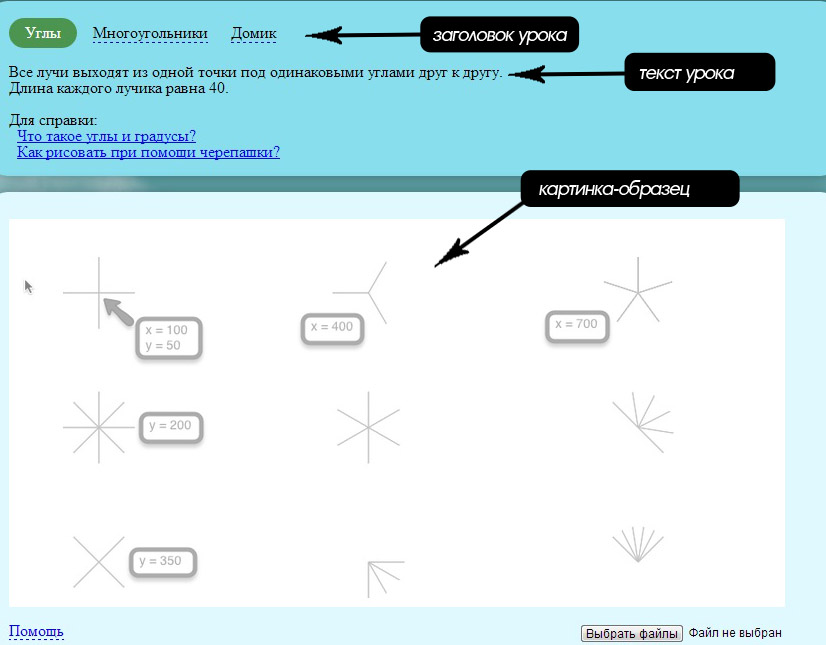
\includegraphics [scale=0.70,natwidth=826,natheight=645] {images/pic1.jpg}
  \caption{Пример урока.} 
  \label{img:pic1}  
\end{figure}


Для создания урока на странице constructor.html в текстовое окно вводится текст урока и, при нажатии кнопки «Создать», содержимое текстового поля извлекается, сжимается, кодируется base64 и создается ссылка на урок.\par
Процесс разработки «Тортуги» ориентирован на то, чтобы программа работала в последних версиях Chrome и Яндекс браузер. Но на данный момент работает и в Fierfox, Safari, IE 8+, Opera, но при возникновении проблем поддержка этих браузеров осуществляется по остаточному принципу.\par
% % % % % % % % % % % % % % % % % % % % % % % % % % % % % % %

\chapter{Конкретные действия поразвитию функционала.} \label{chapt2}

\section{Сокращение ссылки} \label{sect1_1}

Как было сказано выше, сценарий работы с «Тортугой» – это работа с приготовленными уроками, которые открываются по ссылке вида: \par
\vspace{6mm}
\begin{center}
 \textit{ http://tortuga/index.html?b4/wMsYxLAwL/+Ml5/HjEw } (1)\par

\end{center}
\vspace{6mm}

Урок содержит тексты задачи, ссылки на картинки–обазцы, поэтому ссылка получается довольно длинной, например: \par

\begin{center}
\vspace{6mm}
 \textit{ http://tortuga/index.html?7VcxTkMxDL2K9eeqB+gMGys
 TZTCJWywlTkhshIS4O04LN2AA5O3nx35+fk+OkvdNWQ
 tth+2uDarAfVqF3EobMFkBK+kOUpNJSUltAGbuPDmxn
 IEK++6k7BlAbLO2fBSl2j2dJXHmbKJgCgWfvACQXsEJ
 Kp4FAQu/GO7hXoGEq6ND5fXx6kusu6O8GE+QNnVYBnq
 jkVhRuQlYKVhTu0KvIKe1Sl0wuXswEDr36qzaUS5NeD
 Hdw83CRFMCHuZcrv2ywKA+6Jkk0/Dm/cdrK9a9Hjkhb
 xZoTnIoLuVbJu/J4GRnRgVZlKDj8IWNPdy+JepKtrRG
 VpKSMnjknXOqCujyVH6aJxJlpRLLS+brHQE7wLa6eRa
 I2SaNNZubWURwSUSuyLzS1ur+7Dwz1u47TZ28ed2eHi
 P0fxXvs6Rwss4ZsPCsDAs/JET1cPS4L70iZM1xjIs/A
 1j+bGLi2uMZFgYb4/wMsYxLAwL/+Ml5/HjEw== } (2)\par
\end{center}

\vspace{6mm}

Делиться ссылкой такого размера, отправлять по почте, размещать в соц–сетях, использовать в презентациях весьма неудобно. В связи с чем появилась необходимость укорачивания ссылки до 20 знаков и менее. Уже довольно давно существуют способы их сокращения при помощи сайтов–сокращателей таких как:  \textit{www.bitly.com, www.gg.gg, www.goo.gl} и др. Необходимо зайти на соответствующую страницу и после ввода в текстовое окно длинной ссылки, создастся короткая, вида:
 
\begin{center}
\vspace{6mm}
 \textit{ http://goo.gl/fbsS } (3)\par
\end{center}

при переходе по которой происходит перенаправление на длинную. Но такое ручное использование удобно только для единичных вариантов. Что бы создателю уроков не приходилось каждый раз выполнять все эти рутинные операции, возникла задача автоматизировать процесс сокращения ссылок. Для этого было решено воспользоваться API, которое предоставляет Google. Была найдена и использована сторонняя библиотека Jsonlib ~\cite{jsonlib} (автор Девид Бау/David Bau). С ее помощью можно обмениваться запросами в формате JSON технологией AJAX не напрямую, а через сторонний сервер, который осуществляет обращения и возвращает ответ. В связи с чем были созданы функции \textit{getShortenURL} и \textit{parseShortenedResponse}. Одна из которых отправляет запрос с передачей длинной ссылки, а вторая, получив ответ в формате JSON, и, распарсив, выводит на страницу constructor.html в текстовое окно. Если по какой-либо причине запрос не был осуществлен или ответ не был получен, на страницу выводится  длинный URL (см. приложение \ref{AppendixA3} ).


% % % % % % % % % % % % % % % % % % % % % % % % % % % % % % %

\section{Очистка экрана} \label{sect1_1}

При выполнении урока ошибки в алгоритмах рисования неизбежны, и единственный способ очистки экрана - это обновление страницы. Но сраница долго перегружается и приходится заново создавать черепаху с соответствующими настройками положения на экране, ее цветом и толщиной рисования, что отвлекает и создает неудобства. Решением проблемы была бы возможность очистки экрана без обновления страницы. Для этого в библиотеку функций была добавлена еще одна публичная функция \textit{clearCanvas()}, очищающая прямоугольник размером с Canvas (см. приложение \ref{AppendixA3}). Помимо решения такой проблемы очистка экрана дает дополнительные возможности в программировании, например создание анимации.

% % % % % % % % % % % % % % % % % % % % % % % % % % % % % % %
\section{Изменение толщины рисования} \label{sect1_1}

Дополнительное разнообразие достигается при возможности изменения толщины рисования черепахи. Для реализации этого функционала в объект, представляющий черепаху, добавлено свойство width, а в прототип (объект, представляющий свойства и методы, общие для всех черепах) была добавлена функция \textit{setWidth}, внутри которой передаваемая в качестве параметра толщина присваивается конкретной черепахе. Так как доступ к графическому объекту Canvas доступен через графические методы, с помощью которых манипуляции с черепахой отражаются на Canvas, то добавлена открытая функция \textit{setWidth} (см.приложение \ref{AppendixA3}) ~\cite{prototype}.

% % % % % % % % % % % % % % % % % % % % % % % % % % % % % % %
\section{Редактирование урока} \label{sect1_1}

Во время использования созданных уроков возможно выявление  неточностей, ошибок в орфографии и других недочетов, которые требуют исправления. Для этого функционал приложения был дополнен инструментом для редактирования уроков. Для его создания на страницу создания уроков \textit{constructor.html} было добавлено текстовое поле \textit{lessonInput}, в которое вставляется ссылка на уже имеющийся урок. При нажатии на кнопку «Изменить урок» данные из \textit{lessonInput} передаются в свойство \textit{givLessonArea} объекта Tortuga для вызова закрытой функции \textit{updateArea}, которая, в свою очередь,  извлекает текст из ссылки, разархивирует, парсит, и вставляет в текстовое окно в том виде, в котором он был введен. После чего текст урока можно править и далее, при нажатии кнопки «создать урок», формируется новая ссылка на исправленный урок. (см. приложение \ref{AppendixA3}) ~\cite{elementsdom, string}.


% % % % % % % % % % % % % % % % % % % % % % % % % % % % % % %
\section{Вид концов толстых линий} \label{sect1_1}
У большинства детей  слово "программирование" ассоциируется с чем-то сложным, неизвестным, пугающим. Из-за этого интерес к обучению теряется, и задача показать, что программирование это не скучное и нудное, а творческое занятие со множеством решений. Ребенок всегда пытается провести аналогию с тем, что когда либо видел или трогал, и помочь в изучении мы можем дав ему подсказку. Например, показав что рисовать картины можно не только с помощью  кисти, но и программируя действия черепахи, сопоставляя программирование и  кисть -  как инструменты для создания.

Важным элементом рисования является закрашивание объектов, и для этого иногда удобнее использовать линии с прямыми концами, а не скругленными. Например линии с квадратными концами будут создавать видимые изломы на поворотах. А значит, при такой основе как графическое взаимодействие, важно иметь возможность  изменять  концы линий в ходе работы программы. Это добавит гибкости в построении заданий и мышлении ребенка.


Для этого мною. В лексический анализатор  добавлены функции, которые может использовать пользователь для управления черепахой, также пополнил синтаксический анализатор и интерпретатор команд функциями \textit{capsSquare / capsRound и runCapsRound / runCapsSquare} соответственно [приложение А7] и написал вызов команд, работающих с холстом Canvas.

% % % % % % % % % % % % % % % % % % % % % % % % % % % % % %
\section{Изменение урока \# без перезагрузки} \label{sect1_1}


Формирование страниц Тортуги происходит динамически выделением из адресной строки переданных данных, после анализа и обработки которых генерируется страница.
Например 
 
 \begin{center}
 \vspace{6mm}
  \textit{ http://trtg.org/index.html?001nVRNbxJRFP0rL7N /Fw==\#2 }
 \end{center} 
 \vspace{6mm}
 
Если же после построения страницы адресная строка в ходе каких-либо действий изменяется, то для отображения изменений необходимо вновь обработать URL, и  перестроить страницу. Единственным готовым решением является  перезагрузка страницы, но это приводит к сбрасыванию изменений в canvas и дополнительному обращению к серверу, что негативно сказывается на процессе выполнения заданий. 

При изучении данной проблемы оказалось, что современные браузеры отслеживают такое событие как  \textit{onhashchange} - изменение хештега. На основе этого события  можно изменять атрибуты уроков без  обновления страницы, однако для браузеров не поддерживающих \textit{onhashchange} event пришлось использовать таймеры проверки изменений тега.

см. приложение[]

% % % % % % % % % % % % % % % % % % % % % % % % % % % % % % %
\section{Методы изменения координат угла и поворота черепашки} \label{sect1_1}
Во время выполнения урока такой инструмент как черепаха приходится перемещать по всему полю в разные его части, а такие действия возможны только указаниями угла поворота и количестве шагов которые необходимо выполнить. Очевидно этот способ управления требует точности, чем весьма не удобен, и требует отвлекающих подсчетов. Например при начале рисования из определенной точки. По этому было поставлено задание по реализации перемещения черепахи в указанные координаты , а так же поворотом относительно оси OX.

Решена данная проблема следующим образом: на каждом уровне взаимодействия с  черепахой были добавлены функции \textit{setX()} и \textit{setY()},  принимающие координаты точки нового местоположения черепахи по X и по Y  соответственно. А для изменения угла поворота были добавлены методы \textit{setAngle(angle)} и \textit{getAngle()}, устанавливающие и возвращающие угол поворота черепахи в градусах относительно оси OX (против часовой стрелки). 



% % % % % % % % % % % % % % % % % % % % % % % % % % % % % % %
\section{Обработка всех мышинных событий в рамках канвы} \label{sect1_1}

Компьютер стал пользовательским в тот момент, когда появилось взаимодействие с интерфейсом через мышь. Благодаря этому, действия стали интуитивно понятными, что снизило уровень необходимых знаний для использования ЭВМ. Именно по этому большинство детей даже дошкольного возраста пользуются компьютером без чьей либо помощи. Видя этот пример из истории, хотелось бы использовать аналогичное решение для проблемы высокого умственного порога для вхождения в ряды программистов. 

Основой такого шага вперед является возможность отслеживания мышиных событий на canvas, и уже исходя из них должен вызываться им соответствующий механизм обработки. Для этого в файле \textit{DrawingSystem.js}  объекту добавлен  метод \textit{convertCoordsTortugaToCanvas(x, y)}, который получает координаты в Тортужной системе координат, а возвращает объект: \textit{\{x: ?, y: ?\}} - координаты в системе координат canvas, и аналогичный метод \textit{convertCoordsCanvasToTortuga(x, y)}  поступающий в обратном порядке. Это необходимо для  преобразования системы координат canvas  в привычную Декартову. В файле \textit{mouse.js} создал публичный метод \textit{Tortuga.initMouse(drawingSystem)}, и внутри него подписался на все события мыши объекта canvas так, что бы если в глобальном поле \textit{Tortuga.Events} объявлена реакция на произошедшее событие, то оно запускалось. 

Обработка событий мыши на объекте canvas является инструментом  широкого применения для визуализации программы и ее создания при помощи \textit{Drug\&Dropa}.



% % % % % % % % % % % % % % % % % % % % % % % % % % % % % % %
\section{D\&D файлов} \label{sect1_1}
На данный момент выполнение скриптов тротуги выполняется добавлением файла с помощью кнопки "Выбрать файлы" или вводом выполняемого кода непосредственно через консоль браузера.  Было бы весьма удобно обрабатывать скрипты в виде файлов js и просто выделенного куска кода , перемещая их  на страницу тортуги, тем самым ускоряя процесс, не отвлекая школьника от основного занятия.

Современные браузеры отслеживают событие \textit{e.dataTransfer}, использующееся при сохранении данных, перетаскиваемых в его области. Используя API браузера имеем возможность доступа к нему и его обработки. Так как необходимо обрабатывать как файлы, так и выделенный код, перенесенный в специальную область, то в зависимости от типа получаемой информации  происходит ее подготовка, и передача в обработчик скриптов.

% % % % % % % % % % % % % % % % % % % % % % % % % % % % % % %
\chapter{Действия по организации проекта} \label{chapt1}


\section{Автоматизации сборки} \label{sect1_1}

На рынке веб-приложений важно иметь высокую скорость загрузки, а тем более при работе с детьми. Ведь внимание детей трудно удерживать, а пока ожидается реакция браузера ребенок может увлечься посторонними мыслями и потерять как нить рассуждений, так и желание продолжать обучение. 
Во время работы программист использует табуляцию, пробелы и перевод строки, которые пропускаются компилятором при обработке, но важны для создания удобочитаемого и воспринимаемого человеком кода. Это увеличивает размер передаваемых файлов, но допускает возможность их дальнейшей доработки и поиску возникающих ошибок. А значит возникает выбор между уменьшением времени загрузки страницы и удобочитаемостью.

Для ускорения загрузки страницы передаваемые скрипты и css можно минифицировать, но тем самым осложняется отладка продукта, что говорит о неудобстве разработчиков. по этому решением было бы разделение проекта на девелоп и релиз версии.

По этому передо мной стояла задача по автоматизации сборки проекта по общему файлу-шаблону для всех страниц с подключением к каждой странице как стандартного набора скриптов, так и индивидуальных js-файлов соответствующих урокам. Так же иметь возможность подключать как только минифицированные файлы js и css для клиентской release -версии приложения, так и  только исходный удобочитаемый набор файлов для debug-версии разработчиков. Помимо этого уметь сжимать необходимые js -файлы в один файл \textit{min.js} и css-файлы в один \textit{min.css}.

Большинство задач, с которыми приходится сталкиваться программистам, уже давным-давно решены другими членами нашего сообщества. Классическим сборщиком является Make, до сих пор являющийся стандартом де факто при сборке программного обеспечения для Linux из исходников. Это простой, старый и при этом могучий инструмент, до сих пор не утративший своей актуальности, однако требующий умения писать shell - скрипты и пользоваться утилитами Unix, и , что не маловажно, быстро увеличивает рост сложности проекта. В отличие от Make, утилита Ant (Another Neat Tool)  полностью независима от платформы, требуется лишь наличие на применяемой системе установленной рабочей среды Java — JRE. Отказ от использования команд операционной системы и формат XML обеспечивают переносимость сценариев. Имеет встроенные задачи, но их очень мало для фронтенда. Gradle - построен на принципах Apache Ant и Apache Maven, но предоставляющая Предметно-ориентированный язык на основе языка Groovy вместо традиционной XML-образной формы представления конфигурации проекта.

Взрыв инструментов языка JavaScript, помогающих оптимизировать рабочий процесс front - end - разработчиков  перешел далеко за свои пределы. Все основные инструменты, которые используются для тестирования и разработки на JavaScript активно поддерживаются Node.js. Одним из современных продуктов сборки является Grunt. В отличии от других ему подобных инструментов Grunt создавался специально для фронтенд-разработчиков. И сам Грант, и расширения для него, и даже конфиг написаны на знакомом им языке - JavaScript. Этот инструмент пользуется большой популярностью у веб-разработчиков по всему миру и позволяет не только экономить время, избавляя от монотонных задач, но и выполнять то, что раньше автоматически было делать невозможно. В первую очередь нам интересны такие возможности как:


\begin{itemize}
  \item проверка javascript-кода на ошибки;
  \item склеивание и минификация исходников в один файл;
  \item запуск unit-тестов;
  \item отслеживание изменений исходных файлов и автоматический перезапуск необходимых задач;
\end{itemize}


Расширения Grunt продолжают разрабатываться и сегодня, увеличивая его функциональность. Разнообразие его возможностей позволяет подобрать необходимые инструменты и наладить их наиболее подходящим для нашей ситуации образом. Ведь каждое решение по проектированию, которое принимается, будет иметь некоторый набор результатов, в который, как минимум, должно быть включено удовлетворительное решение поставленной задачи. И от этого набора полученных результатов зависит дальнейшая перспектива развития продукта Тортуга. В качестве сборщика был выбран Grunt.

В роли шаблонизатора имеется возможность использовать Assemble, поскольку он позволяет осуществить настройку  таким образом, что сборка страниц может происходить с подключением шаблонов, присущих только некоторому набору страниц, а так же передавать файлы json формата.

Подключение js и css - файлов происходит из разделов src/js и src/css благодаря расширению \textit{sails-linker}, имеющий возможность подключать файлы любого формата в любом шаблоне, и к тому же имеет разные настройки для debug и release версий.

\textit{copy} осуществляет копирование файлов по необходимым разделам , и к тому же имеет возможность изменения 

\textit{uglify} минимизирует и склеивает исходные файлы в min.js и min.css.

\textit{clean} целиком очищает раздел, в который организована сборка проекта.

\textit{watch} автоматически перезапускает сборку проекта при изменении выбранного набора файлов.


Вместе они позволили настроить сборщик Grunt таким образом, что бы при внесении изменений автоматически собирать как release - версии с минифицированными файлами, так и debug - версии.

%\newpage
%============================================================================================================================

\section{Изменение архитектуры} \label{sect1_1}
Изначально рассчитывалось, что Тортуга будет небольшим и скромным приложением, но со временем требования к нему росли. Необходимые усовершенствования и доработка функционала сделали ее несколько более сложной и взаимосвязанной. А значит, что при дальнейшем росте зависимость между ее компонентами будет расти, что повышает актуальность проблемы создания гибкой расширяемой архитектуры. 

Передовые программисты уже не раз сталкивались с подобными задачами, решение которых проанализировано, объяснено, проверено на практике и сформированы общепринятые паттерны проектирования для создания такой архитектуры. Необходимые определения и способы взаимоотношения компонентов воссозданы во фреймворках, и в качестве подходящего мы выбрали AngularJS.

Раньше структура приложения Тортуга была такой. Вызывалась функция initApp(), которая устанавливала зависимости между существующими html-документами, создавала нужные данные и вспомогательные html-элементы, устанавливала обработчики событий. Другими словами вносила логику и устанавливала связи между распределенными по разным файлам частями. Основными компонентами были: контейнер поля с черепахой и контейнер списка задач урока и текстом. Команды, вызванные пользователем либо из консоли, либо из файла, попадают в лексический анализатор, который формирует из них набор лексем, и передает в синтаксический анализатор, перерабатывающий их и строящий дерево программного кода. Команды управления черепахой представляют из себя отдельный язык, не похожий на javascript, по этому дерево кода передается в интерпретатор команд черепахи и с помощью интерфейса рисования отображаются результаты на экране.

\vspace{6mm}
ТУТ СХЕМКА
\vspace{6mm}

В новой же структуре благодаря AngularJS наш сложный initApp() с описанием действий по вызову модулей  и их связям отсутствует. Все компоненты передаются друг в друга за пределами Тортуги, а сама передача осуществляется с помощью Ангуляра, который создает экземпляры и связывает их исходя из зависимостей, описанных в конфигурации.

В шаблоне страницы присутствует тег <tbox\_tortoise\_canvas/>, являющийся директивой  и отвечающий за внешние преобразования, в том числе за размещение дополнительных html-элементов. Эта директива напрямую связана с контроллером, обеспечивающим связь между такими сервисами как Менеджер Мышиных Команд  и Диспетчер Сообщений. Менеджер отвечает за вызов функций, подписанных на определенные события canvas, а Диспетчер Сообщений за поддержку связи модулей Тортуги с контроллером.

TortoiseGlobals - интерфейс пользователя. Он регистрирует все глобальные функции, которые может вызывать пользователь. Полученные им команды передаются в синтаксический анализатор, который строит дерево команд и передает его в интерпретатор - исполнитель дерева команд черепахи, а он, в свою очередь,  связан только с Диспетчером Сообщений, в который отправляет переработанные команды в виде элементарных графических операций.

В диспетчер сообщений фреймворк передает в качестве параметра TortoiseCanvasBlock, который получает сообщения о графических операциях, и исполняет их.

\vspace{6mm}
ТУТ СХЕМКА
\vspace{6mm}

Описав такую зависимость в конфигурационном файле Ангуляр сам объявляет и запускает необходимые компоненты, и отвечает за передачу данных между ними. Использование AngularJS в проекте стандартизировало компоненты и связи между ними с точки зрения фреймворка. Таким образом у нас внедрен инструмент, позволяющий расширять проект и управлять модулями заранее декларированным образом, что делает рост проекта более управляемым.


\clearpage